\chapter{Príklady MITM útokov}
\label{kap:priklady}

V tejto kapitole uvedieme dva príklady použitia FPGA MITM obvodu, ktorého implementáciu sme opísali v kapitole \ref{kap:implementacia}. Prvým bude jednoduchý príklad zasahovania do komunikácie na UART zbernici, na ktorom demonštrujeme detailnejšie celý proces od navrhnutie MITM logiky po zapojenie a spustenie obvodu. Druhým príkladom je útok na funkciu náhodného generátora externého TPM modulu pripojeného k mikrokontroléru ESP8266.

\section{Príklad 1 -- zasahovanie do UART komunikácie} \label{sek:example1}
Ako prvý uvedieme jednoduchý príklad MITM obvodu, ktorý bude zasahovať do UART komunikácie. Cieľom tohoto príkladu je ukázať postup pri implementácii hardvérového MITM útoku s využitím nášho obvodu. FPGA obvodu bude možné prepínať medzi štyrmi režimami, pričom jeden z nich bude transparentný -- žiadne zásahy do komunikácie. V ostatných troch režimoch implementujeme tri rôzne logiky, ktoré budú rozličnými spôsobmi zasahovať do komunikácie. Cieľom je demonštrovať viaceré možnosti, ktoré naša implementácia poskytuje. Najskôr ukážeme detailný návrh MITM logiky, následne konfiguráciu a syntézu FPGA obvodu. Na záver ukážeme fyzické zapojenie hardvéru a spustenie útoku.

\subsection{Návrh MITM logiky} \label{subsek:uartMitmLogic}
Celý návrh MITM logiky sa nachádza v jednom Verilog module, ktorého názov musí byť \texttt{MitmLogic} a jeho definícia sa musí nachádzať v súbore \texttt{MitmLogic.v} v adresári \texttt{src/}. Ako prvé je v module MITM logiky potrebné definovať parametre a vstupy/výstupy. Potrebné je definovať dva parametre. Prvým je \texttt{NUM\_DATA\_BITS} -- veľkosť bloku dát v bitoch. V prípade UART zbernice je táto hodnota štandardne osem bitov. Druhým parametrom je \texttt{NUM\_MITM\_MODES}, ktorý určuje počet rôznych MITM režimov, maximálne sú podporované štyri. V niektorých verziách jazyka Verilog je požadované, aby mali parametre nastavenú predvolenú hodnotu. Na tejto hodnote však nezáleží, nakoľko bude použitá hodnota nastavená v konfigurácii, ktorú ukážeme v ďalšej časti.

Ďalej je potrebné definovať dva systémové vstupy -- systémové hodiny a globálny reset a jeden vstup prichádzajúci z I/O handler modulu, ktorý vždy udržuje hodnotu aktuálne nastaveného MITM režimu. Okrem týchto vstupov je potrebné definovať celé zbernicové rozhranie podľa úryvku \ref{snip:busInterface}, pričom vstupy rozhrania predstavujú výstupy MITM logiky a naopak. Sémantiku týchto vstupov a výstupov sme vysvetlili v časti \ref{sek:busInterface}. Celý zdrojový kód tejto ukážkovej MITM logiky sa nachádza v súbore \texttt{examples/SimpleUartMitmLogic.v} v elektornickej prílohe.

Následne definujeme logiku samotného modulu. V našom prípade chceme podporovať štyri režimy MITM logiky, ktoré zadefinujeme ako lokálne konštanty. Prvým režimom je transparentný režim, kedy do komunikácie nechceme zasahovať. Ten vyriešime jednoduchou logikou -- budeme sledovať vstupný režim z I/O handler modulu. Pokiaľ je nastavený na hodnotu prvého režimu vypneme falošný mód na zbernicovom rozhraní. To spôsobí, že akékoľvek inštrukcie pre posielanie falošných dát na rozhraní budú ignorované. V úryvku \ref{snip:fakeSelect} je ukážka kódu, ktorý realizuje túto logiku.

\begin{lstlisting}[float,language=Verilog,caption={Prepínanie medzi transparantným a falošným režimom MITM logiky.},label=snip:fakeSelect]
always @ (posedge sys_clk)
begin
    // prečítame aktuálne nastavený MITM režim
    mode <= mode_select;

    // ak je nastavený transparentný režim,
    // vypneme falošný režim na rozhraní
    if (mode == MODE_FORWARD) begin
        fake_if0_select <= 1'b0;
        fake_if1_select <= 1'b0;
    end
    // inak, zapne falošný režim na rozhraní
    else begin
        fake_if0_select <= 1'b1;
        fake_if1_select <= 1'b1;
    end
end
\end{lstlisting}

Pre účely falošného režimu budeme sledovať stav komunikácie na jednotlivých rozhraniach. Keďže UART je asynchrónny stav bude nezávislý na oboch stranách. Pre obidva smery komunikácie budeme mať vlastný stavový register, ktorých sémantika bude symetrická. Definujeme nasledovné tri stavy: čítanie \texttt{READ}, zápis \texttt{WRITE} a ukončenie komunikácie \texttt{FINISH}.

V stave \texttt{READ} budeme čakať na signalizáciu zbernicového rozhrania, že boli prečítané nové dáta. Keďže na druhej strane zatiaľ nić neposielame a rozhranie je vo falošnom režime, komunikácia je blokovaná. To nepredstavuje v prípade UART protokolu žiaden problém nakoľko je asynchrónny. Po prečítaní nových dát tieto dáta spracujeme podľa aktuálneho režimu (v jednom takte) a presunieme sa do stavu \texttt{WRITE}.

V stave \texttt{WRITE} počkáme na statusový signál, že zbernicové rozhranie je pripravené na zápis. Následne zapneme riadiaci vstup pre spustenie vysielania falošných dát a presunieme sa do posledného stavu \texttt{FINISH}. V tomto stave počkáme na statusový signál, že dáta boli odvysielané a vrátime sa naspäť do stavu \texttt{READ}. Tento cyklus sa opakuje nezávisle pre obidva smery komunikácie.

V prípade, že v ktoromkoľvek takte bude zapnutý vstup globálny reset, prejdeme do špeciálneho stavu \texttt{RESET}. V stave \texttt{RESET} s nasledujúcim taktom nastavíme interné registre do predvoleného stavu a prejdeme naspäť do počiatočného stavu \texttt{READ}. Na obrázku \ref{obr:mitmStateTransition} je znázornený prechodový diagram stavov MITM logiky pre jeden smer komunikácie.

\begin{figure}
    \centerline{\includegraphics[width=1\textwidth]{images/misc/mitmStateTransition.pdf}}
    \caption[Prechodový diagram stavov MITM logiky]{Prechodový diagram stavov MITM logiky. Znázornený diagram je pre smer komunikácie IF0->IF1. Logika prechodov pre opačný smer je analogická.}
    \label{obr:mitmStateTransition}
\end{figure}

V rámci MITM logiky definujeme okrem transparentného režimu, tri ukážkové falošné režimy. V prvom režime nahrádzame v jednom smere ľubovoľnú hodnotu za konštantu 0x23 (ASCI hodnota znaku \#) a v opačnom smere komunikáciu úplne blokujeme. (V stave \texttt{WRITE} nezapneme signál pre spustenie vysielania.) Ďalší falošný režim bude symetrický, pričom vymeníme smer, v ktorom nahrádzame dáta konštantou, so smerom, v ktorom komunikáciu blokujeme. Ako konštantu budeme tentokrát posielať hodnotu 0x24 (ASCI hodnota znaku \$). V poslednom režime budeme nad vybranými dátami realizovať transformáciu ROT13 oboma smermi. Pokiaľ prečítame hodnotu z rozsahu A--Z alebo a--z, dáta zrotujeme, v opačnom prípade pošleme hodnotu, ktorú sme prečítali.

\subsection{Konfigurácia a syntéza FPGA obvodu}
Ďalej je potrebné nakonfigurovať parametre v súbore \texttt{config.vh}. Najdôležitejším parametrom je frekvencia systémových hodín, ktorého obmedzenia sme spomenuli v časti \ref{subsek:sysFreq}. Pre tento účel je najskôr potrebné určiť symbolovú rýchlosť zbernice UART. V našom prípade budeme používať štandardnú rýchlosť 115\,200, čo v zodpovedá 115.2\,kHz. Táto frekvencia vysielania dát je približná nakoľko UART protokol povoľuje odchýlku 5\%. Frekvenciu systémových hodín nastavíme preto na 16\,MHz, čo je minimálna hodnota, ktorú je použitý PLL obvod schopný generovať. Ďalšie parametre, ktoré je potrebné upraviť sú spomenutá symbolová rýchlosť, počet bitov jedného rámca -- v prípade štandardnej UART komunikácie 8 a počet režimov MITM logiky, ktoré sme v predošlej časti \ref{subsek:uartMitmLogic} definovali štyri. Parametre týkajúce sa SPI zbernice nemusíme konfigurovať. Ostatné parametre ponecháme na predvolenej hodnote. V tabuľke \ref{tab:uartConfig} nakonfigurované hodnoty všetkých relevantných parametrov.

\begin{table}
    \caption[Príklad konfigurácie parametrov pre UART]{Príklad konfigurácie parametrov pre UART.}
    \label{tab:uartConfig}
    \begin{center}
    \begin{tabular}{V{4}c|cV{4}}
        \hlineB{4}
        Parameter & Hodnota \\
        \hlineB{4}
        SYS\_FREQ & 16 \\
        \hline
        DEBOUNCE\_LEN\_US & 50\,000 \\
        \hline
        NUM\_MITM\_MODES & 4 \\
        \hline
        NUM\_DATA\_BITS & 8 \\
        \hline
        UART\_BAUD\_RATE & 115\,200 \\
        \hlineB{4}
    \end{tabular}
    \end{center}
\end{table}

V tomto príklade budeme syntetizovať obvod pre dosku icestick. Fyzické mapovanie vstupov a výstupov ponecháme také ako je predvolené. Toto mapovanie bude dôležité pri fyzickom zapojení FPGA obvodu v ďalšej časti. Následne môžeme spustiť syntézu FPGA obvodu príkazom \texttt{make icestick-uart}. Skript po úspešnej syntéze vygeneruje v adresári \texttt{build/bin/} binárny súbor s názvom \texttt{icestick-uart.bin}, ktorý možno nahrať na FPGA dosku pomocou programu iceprog. Postup pri nahraní konfigurácie na FPGA závisí od použitého operačného systému a nainštalovaného ovládača pre FPGA dosku.

\subsection{Fyzické zapojenie hardvéru}
Po nahraní konfigurácie na FPGA je potrebné správne zapojiť hardvérové komponenty k FPGA doske -- jednotlivé vodiče použitej zbernice (v našom prípade UART) a tlačidlá pre globálny reset a zmenu MITM režimu. Výstupné LED diódy sa nachádzajú priamo na doske, v prípade potreby je však možné upraviť mapovanie fyzických výstupov a pripojiť vlastné LED diódy k zvoleným výstupom.

Pre demonštráciu funkčnosti implementovanej MITM logiky použijeme dva prevodníky z USB na UART, ktoré pripojíme k počítaču a budeme simulovať komunikáciu pomocou sériového terminálu. Nižšie uvádzame kompletný zoznam použitého hardvéru:
\begin{itemize}
    \item FPGA vývojová doska iCEstick Evaluation Kit
    \item dva prevodníky medzi USB a UART s čipom CP2102
    \item kontaktné bez-spájkové pole
    \item dve spínacie tlačidlá
    \item prepojovacie kábliky
\end{itemize}
Hardvér zapojíme podľa schémy na obrázku \ref{obr:schemeUartMitm}.

\begin{figure}
    \centerline{\includegraphics[width=1\textwidth]{images/schematics/schemeUartMitm.png}}
    \caption[Schéma zapojenia FPGA MITM obvodu pre UART]{Schéma zapojenia FPGA MITM obvodu pre UART.}
    \label{obr:schemeUartMitm}
\end{figure}

Funkcionalitu môžeme následne demonštrovať na jednoduchom scenári: USB konce prevodníkov pripojíme k všeobecnému počítaču. Zároveň zapojíme cez USB aj samotnú dosku icestick kvôli napájaniu (Dátová komunikácia medzi PC a doskou icestick už nie je potrebná, nakoľko FPGA konfiguráciu sme na dosku nahrali v predošlom kroku.) Následne môžeme otvoriť dva virtuálne sériové terminály pripojené k USB prevodníkom. V transparentnom režime MITM logiky sa všetok vstup do prvého terminálu zobrazí na druhom (a naopak). Prepínaním medzi režimami MITM logiky pomocou príslušného tlačidla možno vidieť realizáciu zásahov do komunikácie pri rôznych režimoch, ktoré sme opísali v časti \ref{subsek:uartMitmLogic}.

\section{Príklad 2 -- útok na komunikáciu s TPM} \label{sek:example2}
V tejto časti predstavíme o niečo komplexnejší útok na komunikáciu medzi mikrokontrolérom a externým TPM modulom. Na mikrokontroléri implementujeme program, ktorý bude periodicky získavať náhodne generované dáta pomocou TPM. Následne medzi TPM a mikrokontrolér zapojíme náš FPGA obvod, na ktorom implementujeme MITM logiku, ktorá bude modifikovať náhodne vygenerované bajty, napríklad za konštantné. Konkrétne použijeme mikrokontrolér ESP8266, ktorý bude cez FPGA pripojený k TPM modulu SLB9670.

\subsection{TPM SPI protokol} \label{subsek:tpmSpi}
TPM štandard presne definuje spôsob komunikácie s TPM v prípade, že je použitá zbernica SPI \cite{tpmTis}. V tejto časti uvedieme niektoré detaily zo štandardu, relevantné pre porozumenie princípu útoku na generovanie náhodných čísel. TPM je v role slave zariadenia a komunikáciu riadi druhá strana. Počas SPI komunikácie je počet prenesených bitov (a teda hodinových taktov na SCLK linke) vždy zarovnaný na celý bajt. Bity v rámci bajtu sú vždy prenášané od najvýznamnejšieho bitu a rovnako v prípade viac-bajtových hodnôt sú bajty prenášané od najvýznamnejšieho. Štandard zároveň vynucuje použitie SCLK módu 0.

Na vyššej úrovni komunikácia s TPM prebieha čítaním a zápisom do špecifických TPM registrov. Čítanie a zápis do registra potom vyzerá nasledovne: Najvýznamnejší bit prvého bajtu (posielaný mastrom na MOSI linke) určuje či ide o operáciu čítania (1) alebo zápisu (0). Nasledovných sedem bitov predstavuje počet bajtov, ktoré chceme zapísať/prečítať mínus jeden. Napríklad 0x80 znamená, že chceme prečítať jeden bajt. Nasledujú tri bajty, ktoré určujú adresu registra.

V prípade, že ide o operáciu zápisu po adrese nasledujú jednotlivé dáta, ktoré sa do registra majú zapísať. V prípade operácie čítania je potrebné ďalej taktovať na SCLK linke dostatočný počet bajtov, aby malo TPM priestor odpovedať. V princípe to znamená \uv{poslať} príslušný počet bajtov, na ktorých hodnote nezáleží a podstatné sú iba dáta vysielané z TPM po MISO linke.

Počas posledného bitu (taktu na SCLK linke) adresy registra musí TPM za normálnych okolností transakciu potvrdiť, tým, že dvihne MISO linku na úroveň logickej 1 (efektívne pošle bajt s hodnotou 0x01), tzv. acknowledge (ack). Pokiaľ tak neurobí, uplatní tzv. wait-state podmienku, čím signalizuje, že TPM ešte nie je pripravené posielať/prijímať dáta. Pokiaľ TPM uplatní wait-state podmienku, musí master taktovať ďalšie bajty na SCLK linke, kým TPM nepošle ack. S nasledujúcim bajtom možno začať čítať/zapisovať dáta z/do TPM registra ako v predošlom prípade. V prípade, že už bol úspešne prečítaný/zapísaný aspoň jeden bajt transakcie, TPM nesmie uplatniť ďalšie wait-state podmienky do ukončenia transakcie. Na obrázku \ref{obr:tpmRW} je znázornená komunikácia pri čítaní a zápisu do TPM registra.

\begin{figure}
    \centering
    \subfloat[Prečítanie dvoch bajtov (0x8001) z registra 0xD40024.]{\includegraphics[width=1\textwidth]{images/signals/tpmRead.pdf}}
    \vfill
    \subfloat[Prečítanie dvoch bajtov (0x8001) z registra 0xD40024 s wait-state podmienkou.]{\includegraphics[width=1\textwidth]{images/signals/tpmReadWait.pdf}}
    \vfill
    \subfloat[Zápis jedného bajtu (0xA0) do registra 0xD40018.]{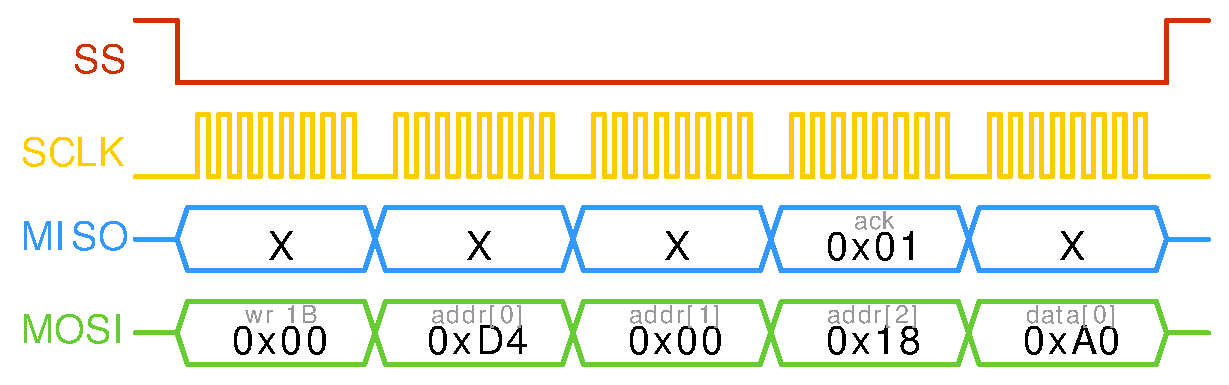
\includegraphics[width=1\textwidth]{images/signals/tpmWrite.pdf}}
    \vfill
    \subfloat[Zápis jedného bajtu (0xA0) do registra 0xD40018 s dvojnásobnou wait-state podmienkou.]{\includegraphics[width=1\textwidth]{images/signals/tpmWriteWait.pdf}}
    \caption[Komunikácia s TPM]{Komunikácia s TPM.}
    \label{obr:tpmRW}
\end{figure}

\subsection{TPM komunikácia na vyššej úrovni}
Jednotlivé registre sú adresované tzv. ofsetom od bázovej adresy. Bázová adresa sa na platformách zvykne využívať na zabezpečenie správneho mapovania TPM registrov do pamäte v prípade použitia memory mapped I/O. V našom jednoduchom prípade na bázovej adrese nezáleží, podstatné je aby počas celej komunikácie bola konštantná. Pre účely tejto práce spomenieme dva podstatné registre.

\textbf{TPM STATUS} register obsahuje statusové aj kontrolné bity, ktoré majú rozličný význam. Niektoré z nich spomenieme v nasledujúcej časti, pri vysvetlení komunikácie s TPM na úrovni príkazov a odpovedí. Pre kompletný zoznam bitov STATUS registra odkazujeme čitateľa na príslušný štandard, ktorý je voľne dostupný \cite{tpmTis}. Hodnoty statusových bitov možno získať prečítaním STATUS registra. Pre nastavenie kontrolných bitov je potrebné zapísať do statusového registra hodnotu, ktorá ma nastavený práve jeden bit (príslušný bit, ktorý chceme nastaviť). Nie je možné nastaviť viacero kontrolných bitov naraz.

\textbf{TPM FIFO} register je základný register na vykonávanie TPM príkazov a získavanie odpovedí. Dátové bajty príkazu pre TPM sa posielajú zápisom do tohto registra. Po vykonaní príkazu možno zase z FIFO registra prečítať dáta TPM odpovede.

Interakciu zadávania príkazov TPM možno opísať stavovým automatom. Po restovaní je TPM v stave \texttt{IDLE}. Pre vykonanie príkazu je najskôr potrebné nastaviť kontrolný bit \texttt{cmdReady} v STATUS registri. Tým prejde TPM do stavu \texttt{READY}. Následne možno postupne zapísať dáta príkazu do FIFO registra. Zápisom prvého bajtu do FIFO registra TPM prejde do stavu \texttt{COMMAND RECEPTION}. Po odoslaní celého príkazu do FIFO registra je potrebné počkať, kým bude v STATUS registri nastavený bit \texttt{stsValid} a zároveň vynulovaný bit \texttt{expect}. Tento status signalizuje, že TPM neočakáva ďalšie príkazové dáta a možno príkaz vykonať. To možno urobiť nastavením kontrolného bitu \texttt{tpmGo} v STATUS registri. Po tomto zápise sa spustí vykonávanie príkazu a TPM prejde do stavu \texttt{COMMAND EXECUTION}.

Po vykonaní príkazu TPM prejde do stavu \texttt{COMMAND COMPLETION}. To možno overiť prečítaním STATUS registra. Je potrebné, aby boli súčasne nastavené bity \texttt{stsValid} a \texttt{dataAvail}, čo signalizuje, že FIFO register obsahuje pripravené dáta odpovede. Následne možno prečítať dáta z FIFO registra. Po prečítaní dát je potrebné opäť nastaviť  bit \texttt{cmdReady} v STATUS registri, čím TPM prejde do stavu \texttt{IDLE}. V stavoch \texttt{COMMAND RECEPTION}, \texttt{COMMAND EXECUTION}, \texttt{CMD COMPLETION} možno kedykoľvek príkaz abortovať nastavením bitu \texttt{cmdReady}, čo spôsobí, že TPM prejde do stavu \texttt{IDLE}. Prechodový diagram TPM stavov je na obrázku \ref{obr:tpmStateTransition}.

\begin{figure}
    \centerline{\includegraphics[width=1\textwidth]{images/misc/tpmStateTransition.pdf}}
    \caption[Prechodový diagram stavov TPM]{Prechodový diagram stavov TPM.}
    \label{obr:tpmStateTransition}
\end{figure}

\subsection{MITM logika pre útok na náhodný generátor TPM}
Podobne ako v príklade 1 (pozri časť \ref{sek:example1}), implementujeme tentokrát mierne zložitejšiu MITM logiku, ktorá bude útok realizovať. Princíp logiky bude spočívať v tom, že budeme detegovať čítanie z FIFO registra. Zo samotnej TPM odpovede nemožno jednoznačne určiť s akým príkazom je odpoveď spätá. Pre jednoduchosť budeme predpokladať, že čítané dáta sú odpoveďou na príkaz \texttt{TPM2\_GetRandom} -- generovanie náhodných čísel. Pre demonštráciu je to postačujúce, nakoľko testovací program pre mikrokontrolér, na ktorom MITM útok demonštrujeme bude po inicializácii TPM vykonávať už len tento jeden príkaz. Počas inicializácie je nutné vykonať aj ďalšie príkazy (\texttt{\_TPM\_Init} a \texttt{TPM2\_Startup}). Pre tento účel budeme mať jeden špeciálny pasívny režim MITM logiky, v ktorom do komunikácie nezasahujeme.

Stavový diagram MITM logiky potom bude vyzerať nasledovne: Začíname v stave \texttt{WAIT\_TPM\_RW}, kedy čakáme na inštrukciu čítania/zápisu z/do TPM registra. Zatiaľ zbernicu ponecháme v transparentnom režime (komunikácia sa preposiela bez zmeny). Po odpočutí 4 bajtoch inštrukcie (kód a adresa registra) prejdeme do stavu \texttt{MITM\_FORK}. Prípadne, pokiaľ TPM uplatnilo wait-state podmienku, prejdeme najskôr do stavu \texttt{TPM\_WAIT\_STATE}, kde počkáme, kým TPM neodpovie ack a následne prejdeme do stavu \texttt{MITM\_FORK}. V stave \texttt{MITM\_FORK} urobíme hlavné rozhodnutie: Na základe odpočutej inštrukcie prejdeme buď do stavu \texttt{MITM\_ATTACK} -- inštrukcia je čítanie z FIFO registra a MITM logika nie je v pasívnom režime, alebo do stavu \texttt{MITM\_IGNORE} v opačnom prípade. Pokiaľ je MITM V stave \texttt{MITM\_IGNORE} nezasahujeme do komunikácie a počkáme až TPM transakcia skončí. Následne sa vrátime do stavu \texttt{WAIT\_TPM\_RW}. Ako ukážku uvádzame v úryvku \ref{snip:tpmRwState} kód realizujúci logiku stavu \texttt{WAIT\_TPM\_RW}. Kompletný zdrojový kód MITM logiky sa nachádza v elektronickej prílohe priloženej k práci.

\begin{lstlisting}[float,language=Verilog,caption={Logika stavu \texttt{WAIT\_TPM\_RW}.},label=snip:tpmRwState]
STATE_WAIT_TPM_RW: begin
    // odpočutie dát na master strane
    if (if0_recv_new_data == 1'b1) begin
        tpm_rw_cmd <= {tpm_rw_cmd[23:0], real_if0_recv_data};
        if0_tpm_rw_ctr <= if0_tpm_rw_ctr + 1;
    end
    // odpočutie dát na slave strane
    if (if1_recv_new_data == 1'b1) begin
        tpm_wait_state <= real_if1_recv_data;
        if1_tpm_rw_ctr <= if1_tpm_rw_ctr + 1;
    end
    
    // ak sme videli 4 bajty (hlavička transakcie), spracujeme ich
    if (if0_tpm_rw_ctr == 3'd4 && if1_tpm_rw_ctr == 3'd4) begin
        if0_tpm_rw_ctr <= 3'd0;
        if1_tpm_rw_ctr <= 3'd0;
        // TPM uplatnilo wait-state podmienku
        // prejdeme do príslušného stavu
        if (tpm_wait_state == 8'h00) begin
            state <= STATE_TPM_WAIT_STATE;
        end
        // v opačnom prípade extrahujeme počet bajtov, ktoré sa budú
        // čítať/zapisovať a prejdeme do ďalšieho stavu
        else begin
            tpm_rw_size <= {1'b0, tpm_rw_cmd[30:24]} + 1;
            state <= STATE_MITM_FORK;
        end
    end
end
\end{lstlisting}

V stave \texttt{MITM\_ATTACK} budeme postupne počítať bajty TPM odpovede na príkaz \texttt{TPM2\_GetRandom}. Prvých desať bajtov budeme pre jednoduchosť ignorovať, nakoľko obsahujú hlavičku s pre nás nepodstatnými informáciami. Bajty 11 a 12 predstavujú počet náhodne vygenerovaných bajtov a túto hodnotu si uložíme. Nasledujú samotné náhodné bajty, ktoré budeme modifikovať na základe režimu MITM logiky. Potom, čo je z FIFO registra prečítaná celá odpoveď, vrátime sa do počiatočného stavu \texttt{WAIT\_TPM\_RW}.

Mikrokontrolér môže TPM FIFO register čítať postupne po menších častiach (min. jeden bajt na transakciu, pozri časť \ref{subsek:tpmSpi}). Uprostred spracovania bajtov čítaných z TPM FIFO registra môže preto dôsť k ukončeniu transakcie. Tento stav vieme detegovať tak, že budeme počítať prečítané bajty. Počet bajtov, ktoré sa majú prečítať zistíme z argumentu inštrukcie čítania. Ak sú všetky bajty prečítané a odpoveď ešte nie je kompletná prejdeme opäť do stavu \texttt{WAIT\_TPM\_RW}, pričom si zapamätáme počet spracovaných bajtov odpovede, aby sme počas ďalšej transakcie vedeli pokračovať.

Z technických dôvodov budeme potrebovať ešte dva stavy \texttt{FAKE\_SEND\_START} a \texttt{STATE\_FAKE\_SEND\_WAIT}, ktoré budú slúžiť na spustenie vysielania falošných dáta a následné čakanie na ich odvysielanie. Posledným stavom je \texttt{RESET}, ktorý slúži na obnovenie počiatočného stavu v prípade globálneho resetu FPGA obvodu, rovnako ako v príklade 1 (pozri časť \ref{sek:example1}). Prechodový diagram stavov MITM logiky pre útok na náhodný generátor TPM je na obrázku \ref{obr:tpmMitmStateTransition}.

\begin{figure}
    \centerline{\includegraphics[width=1\textwidth]{images/misc/tpmMitmStateTransition.pdf}}
    \caption[Prechodový diagram stavov MITM logiky pre útok na TPM]{Prechodový diagram stavov MITM logiky pre útok na TPM. Z každého stavu vedie prechod na globálny reset do \texttt{RESET} stavu. Kvôli prehľadnosti sú tieto prechody vynechané.}
    \label{obr:tpmMitmStateTransition}
\end{figure}

\subsection{Demonštrácia útoku}
Pre demonštráciu útoku sme naprogramovali jednoduchý program pre mikrokontrolér ESP8266 na doske NodeMCU, ktorý komunikuje s TPM modulom SLB9670. Program po inicializovaní TPM, periodicky posiela príkaz na generovanie náhodných bajtov a následne vždy prečíta odpoveď, ktorú vypíše cez UART pripojený napríklad k virtuálnemu terminálu počítača. Program sme implementovali v prostredí Arduino IDE a zdrojový kód sa nachádza v elektronickej prílohe priloženej k práci.

Opäť je potrebné správne nakonfigurovať parametre FPGA obvodu, ktoré závisia aj od nastavení SPI zbernice použitej na komunikáciu. Parametre, ktoré sme zvolili pre demonštráciu útoku sú v tabuľke \ref{tab:tpmConfig}. Narozdiel od predošlého príkladu (časť \ref{sek:example1}), v tomto príklade použijeme dosku iCE40-HX8K, pričom fyzické mapovanie vstupov a výstupov ponecháme predvolené. Syntézu Verilog kódu v tomto prípade spustíme príkazom \texttt{make ice40hx8k-spi} a výsledný súbor \texttt{ice40hx8k-spi.bin} nahráme na FPGA dosku pomocou programu iceprog, rovnako ako v prvom príklade. Pre demonštráciu útoku sme použili nižšie uvedený hardvér, ktorý sme zapojili podľa schémy na obrázku \ref{obr:schemeTpmMitm}.
\begin{itemize}
    \item FPGA vývojová doska iCE40-HX8K Breakout Board
    \item vývojová doska NodeMCU ESP8266
    \item TPM module SLB9670
    \item kontaktné bez-spájkové pole
    \item dve spínacie tlačidlá
    \item prepojovacie kábliky
\end{itemize}

\begin{table}
    \caption[Konfigurácia parametrov pre útok na TPM]{Konfigurácia parametrov pre útok na TPM.}
    \label{tab:tpmConfig}
    \begin{center}
    \begin{tabular}{V{4}c|cV{4}}
        \hlineB{4}
        Parameter & Hodnota \\
        \hlineB{4}
        SYS\_FREQ & 60 \\
        \hline
        DEBOUNCE\_LEN\_US & 50\,000 \\
        \hline
        NUM\_MITM\_MODES & 4 \\
        \hline
        NUM\_DATA\_BITS & 8 \\
        \hline
        SPI\_FREQ\_HZ & 1\,000\,000 \\
        \hline
        SPI\_SS\_ACTIVE\_LOW & 1 \\
        \hline
        SPI\_LSB\_FIRST & 0 \\
        \hlineB{4}
    \end{tabular}
    \end{center}
\end{table}

\begin{figure}
    \centerline{\includegraphics[width=1\textwidth]{images/schematics/schemeTpmMitm.png}}
    \caption[Schéma zapojenia hardvéru pre útok na TPM]{Schéma zapojenia hardvéru pre útok na TPM.}
    \label{obr:schemeTpmMitm}
\end{figure}

Po zapojení hardvéru a spustení možno pozorovať, že program z TPM korektne získava náhodne generované bajty -- MITM logika FPGA je v pasívnom režime. Po stlačení tlačidla mode select možno pozorovať, že prečítané \uv{náhodné} bajty, ktoré program na mikrokontroléri vypisuje nemajú vlastnosti náhodne generovaných dát. V závislosti od nastaveného režimu MITM logiky sú napríklad konštantné, alebo sú postupne inkrementované o 1.

\subsection{Technické nedostatky}
Pri realizácii tohoto útoku sme zároveň pozorovali občasné zlyhanie komunikácie medzi mikrokontrolérom a TPM. Toto zlyhanie bolo s najväčšou pravdepodobnosťou spôsobené nízkou kvalitou vodivého prepojenia (pomocou káblikov) medzi komponentami. Najproblematickejším spojením bola linka SCLK, ktorá prenáša hodinový signál. Pri vyšších frekvenciách (rádovo viac ako 10\,MHz) SPI zbernicene, sme pozorovali mierne odlišnosti medzi SCLK signálom vysielaným mikrokontrolérom a signálom, ktoré generovalo FPGA. Tieto výchylky mohli spôsobiť nestabilitu komunikácie. 

Pre stabilnejšiu komunikáciu by bolo potrebné použiť kvalitnejšie prepojenie medzi elektronickými súčiastkami, napríklad pomocou vhodnej dosky plošných spojov. Cieľom tohto príkladu bolo iba konceptuálne demonštrovať možnosť použitia nášho FPGA obvodu na realistickejšie útoky. Optimalizácia podobných technických aspektov je preto mimo rozsah tejto práce a považujeme ju za jednu z možností nadviazania na túto prácu.